\documentclass[border=10pt]{standalone}

\usepackage{tikz}
\usepackage{tikzsymbols}
\usetikzlibrary{calc,patterns,shapes.geometric}

\def\centerarc[#1](#2)(#3:#4:#5){\draw[#1] ($(#2)+({#5*cos(#3)},{#5*sin(#3)})$) arc (#3:#4:#5);}

\begin{document}
	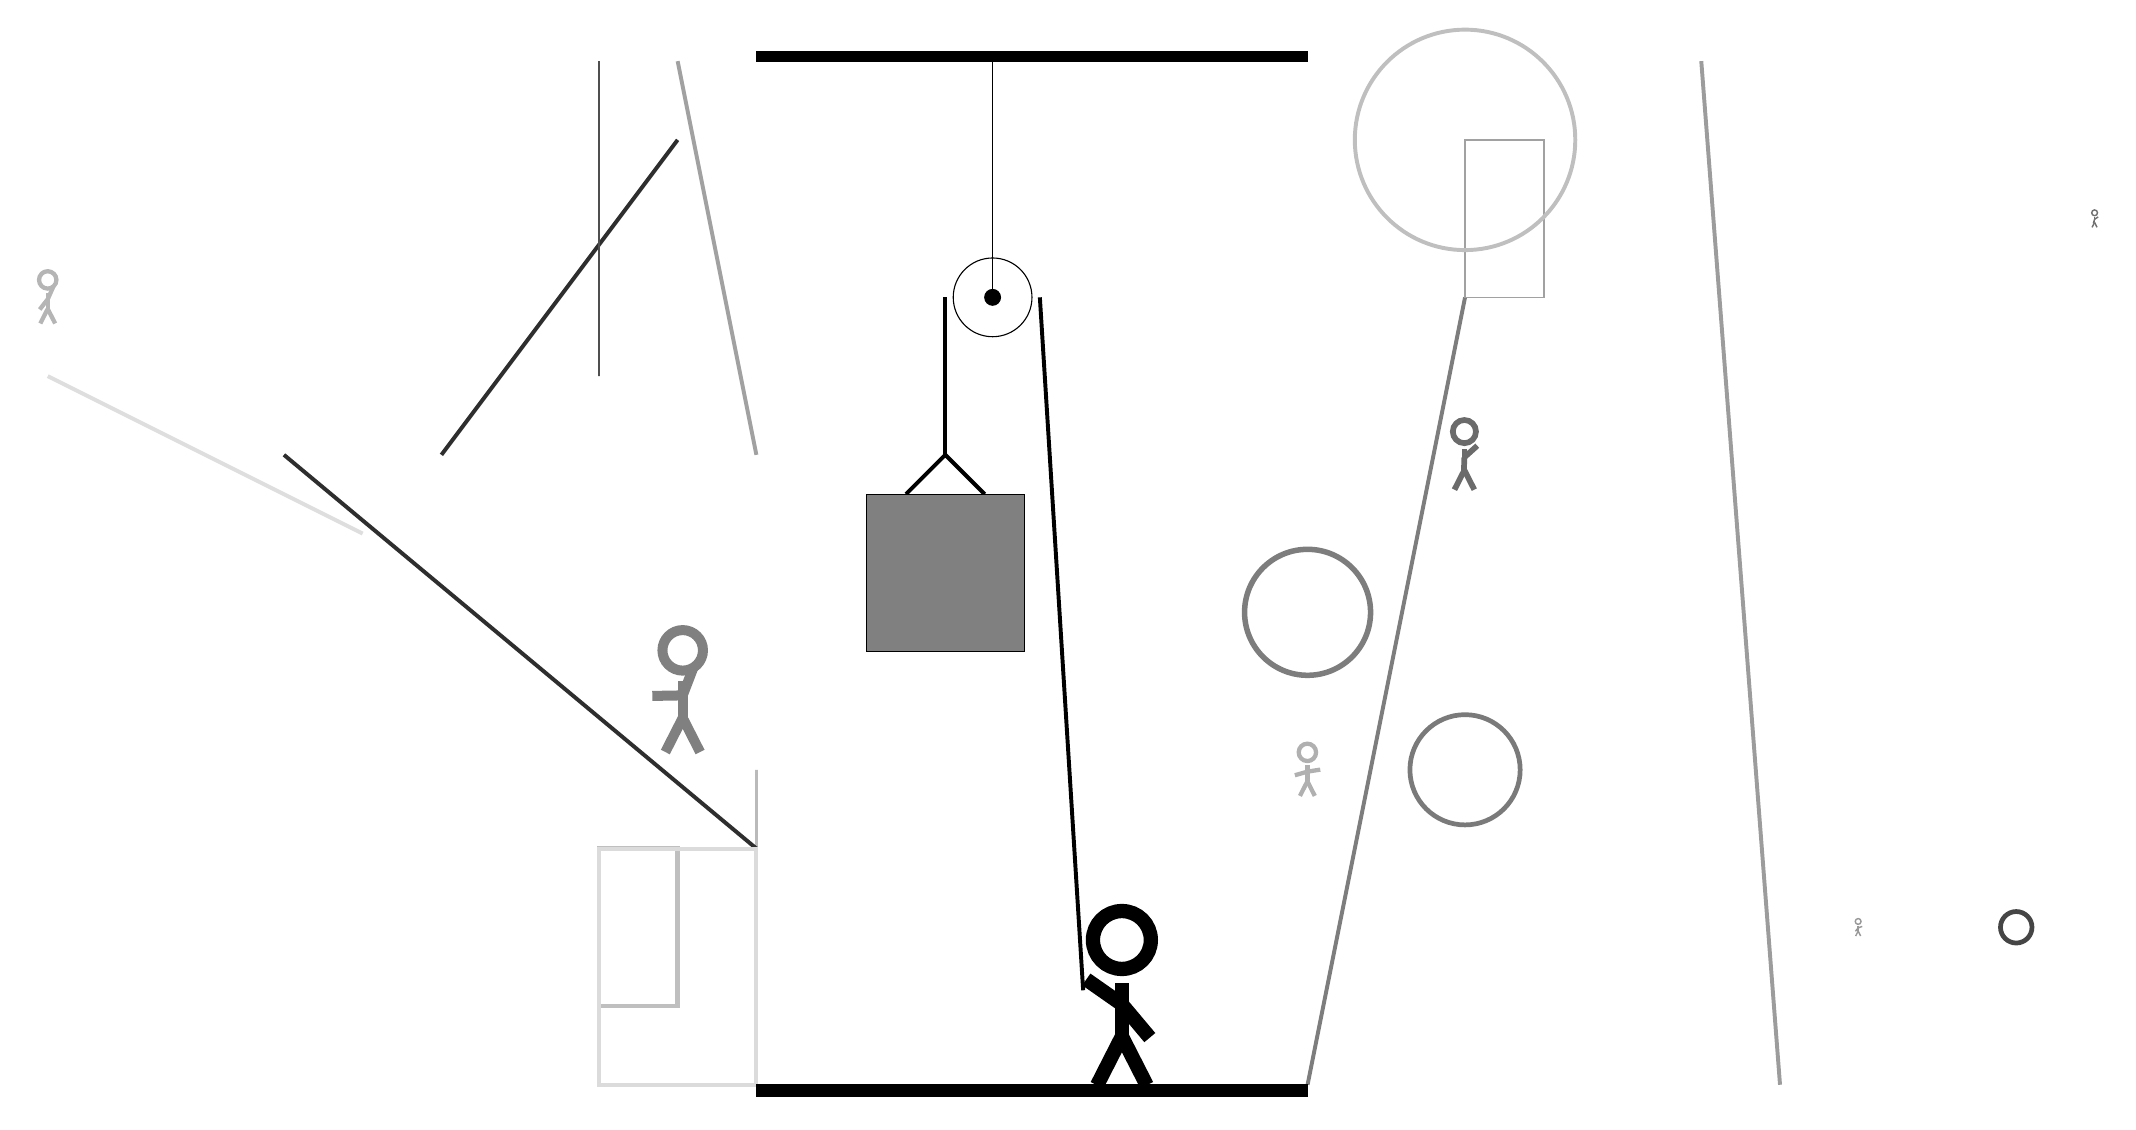
\begin{tikzpicture}
		%%%%% START %%%%%
		
		\draw[fill=black] (-2, 10) rectangle (5, 10.125);
		
		\draw (1, 7) circle (0.5);
		\draw[fill=black] (1, 7) circle (0.1);
		\draw (1, 10) -- (1, 7);
		
		\draw[line width=0.5mm] (-0.1, 4.5) -- (0.4, 5.0) -- (0.9, 4.5);
		\draw[fill=black!50] (-0.6, 4.5) rectangle (1.4, 2.5);
		
		\draw[line width=0.5mm] (0.4, 7) -- (0.4, 5.0);
		\centerarc[line width=0.5mm](1, 7)(0:180:0.6);
		\draw[line width=0.5mm](1.6, 7) -- (2.15, -1.8);
		
		\node[line width=0.5mm, color=black!58] at (7, 5) {\Strichmaxerl[4][88][42]};
		
		\draw[line width=0.3mm, color=black!27] (-2, -2) rectangle (-2, 1);
		\draw[line width=0.5mm, color=black!82](-3, 9) -- (-6, 5);
		\draw[line width=0.2mm, color=black!69] (-4, 10) rectangle (-4, 6);
		\draw[line width=0.6mm, color=black!25] (-4, -2) rectangle (-3, 0);
		
		\draw[line width=0.5mm, color=black!51](7, 7) -- (5, -3);
		\draw[line width=0.5mm, color=black!13](-7, 4) -- (-11, 6);
		\draw [line width=0.6mm, color=black!52](7, 1) circle (0.7);
		\draw[line width=0.5mm, color=black!82](-2, 0) -- (-8, 5);
		\node[line width=0.3mm, color=black!29] at (-11, 7) {\Strichmaxerl[3][52][66]};
		\draw[line width=0.2mm, color=black!37] (7, 7) rectangle (8, 9);
		
		\draw [line width=0.6mm, color=black!73](14, -1) circle (0.2);
		\node[line width=0.4mm, color=black!56] at (15, 8) {\Strichmaxerl[1][73][33]};
		\draw [line width=0.6mm, color=black!41](13, 1) circle (0.0);
		\draw[line width=0.5mm, color=black!37](-2, 5) -- (-3, 10);
		\node[line width=0.6mm, color=black!50] at (-3, 2) {\Strichmaxerl[7][1][69]};
		\draw [line width=0.7mm, color=black!51](5, 3) circle (0.8);
		\draw[line width=0.5mm, color=black!39](10, 10) -- (11, -3);
		\draw [line width=0.5mm, color=black!25](7, 9) circle (1.4);
		\node[line width=0.3mm, color=black!40] at (12, -1) {\Strichmaxerl[1][51][20]};
		\node[line width=0.7mm, color=black!31] at (5, 1) {\Strichmaxerl[3][16][9]};
		
		\draw[line width=0.5mm, color=black!14] (-4, -3) rectangle (-2, 0);
		
		\node at (2.6, -1.9) {\Strichmaxerl[10][-35][-50]};
		
		\draw[fill=black] (-2, -3) rectangle (5, -3.15);
		
		%%%%% END %%%%%
	\end{tikzpicture}
\end{document}